\chapter{Installation et configuration d'un client git}
Pour commencer : nous allons apprendre à utiliser un client git.
Pour ce tutoriel, vous devrez avoir un compte sur \href{https://github.com/}{Github}.

\section{Installation}
\subsection{Windows}

Pour Windows, nous allons parler de deux alternatives :

\begin{itemize}
	\item Utiliser la console
	\item Utiliser une interface simplifiée\\
\end{itemize}


Puisque tout au long du tutoriel, nous allons voir les deux en même temps, nous allons les installer tous les deux.\\

Téléchargez et installez donc :
\begin{enumerate}
	\item \href{http://msysgit.github.io/}{msysgit} (git pour windows)
	\item \href{http://code.google.com/p/tortoisegit/wiki/Download}{tortoise git} (une interface simplifiée).\\
\end{enumerate}

\textbf{Attention !}
Durant l'installation on vous demandera de choisir le style de fin de ligne durant les commits/checkout et si les commandes doivent se mettre dans le PATH.\\

\begin{itemize}
	\item Pour les fins de lignes : laissez le choix par défaut (checkout windows, commit unix)
	\item Pour le choix des outils du path : choisissez d'ajouter git et seulement git au path (seconde option)
\end{itemize}
\newpage
\subsection{Unix}

Vous n'aurez pas d'interface ici (mis à part git gui), vous devrez principalement utiliser le terminal.
Commencez par installer git, par ici : \href{http://code.google.com/p/git-osx-installer}{Installer}\\

Il existe deux interfaces simplifiées, par défaut : gitk et git gui (qui communiquent)

\subsection{GNU/Linux}
Il vous suffit d'utiliser le gestionnaire de paquet de votre distribution
\subsubsection{Debian-like}
\begin{verbatim}
> apt-get install git
\end{verbatim}
\subsubsection{Fedora}
\begin{verbatim}
> yum install git-core
\end{verbatim}

Il existe deux interfaces simplifiées, par défaut : gitk et git gui (qui communiquent)

\section{Configuration du client}
\subsection{Générer la clé SSH}
\subsubsection{Par git gui}

Certains dépôts git fonctionnent avec une clé SSH, ce qui permet de sécuriser la connection.
Pour générer une clé SSH, nous allons utiliser git gui :

\begin{itemize}
	\item Ouvrez git gui
	\item Menu Aide
	\item Montrer la clé SSH
	\item (si aucun texte n'est affiché) Générer la clé
	\item Copier la clé dans le presse papier\\
\end{itemize}

\subsubsection{Par commande}

\begin{verbatim}
	# Pour voir les clés déjà existantes
	$ cd ~/.ssh
	$ ls
	
	# Pour générer une clé
	$ ssh-keygen -t rsa -C "email@example.com"
	
	# Pour tester si la clé marche
	$ ssh -T git@github.com
\end{verbatim}

\newpage
\subsection{Donner la clé à Github}

Nous allons maintenant prendre cette clé et la lier au serveur git (ici : github)\\
Pour cela :

\begin{itemize}
	\item Connectez-vous
	\item Allez dans Account settings
	\item SSH Keys
	\item Add SSH key
	\item Collez la clé dans le champs texte "Key" et validez "Add key".
\end{itemize}

Emplacement des Account settings :

\begin{figure}[h] 
	\begin{center}
		
\includegraphics[scale=0.5]{../IMG/githubsettings.jpg}
	\end{center}
	\caption{GitHub : les reglages}
	\label{GitHub : les reglages} 
\end{figure}

\subsection{Les informations d'utilisateurs}

Plusieurs serveurs ssh demandent à savoir deux-trois choses sur vous : l'identification ssh ou par login
ne suffit pas. Il faut aussi identifier le client.

\subsubsection{Par fichier}

Dans votre HOME, vous devriez trouver un fichier .gitconfig (caché).
Celui-ci doit contenir plusieurs préférences pour votre client git, dont : l'identification du client dans la clause [user].
Si celle-ci n'existe pas, vous allez devoir la créer :

\begin{verbatimtab}[4]
[user]
	name = Votre nom
	email = email@example.com

\end{verbatimtab}

\subsubsection{Par commande}

\begin{verbatim}
	$ git config --global user.name "Votre nom"
	$ git config --global user.email "email@example.com"
\end{verbatim}
\newpage
\subsubsection{Par Tortoise Git}
Commencez par faire un clic droit, n'importe où : vous voyez que plusieurs options ont été ajoutées : il s'agit de tortoise git.

\begin{figure}[h] 
	\begin{center}
		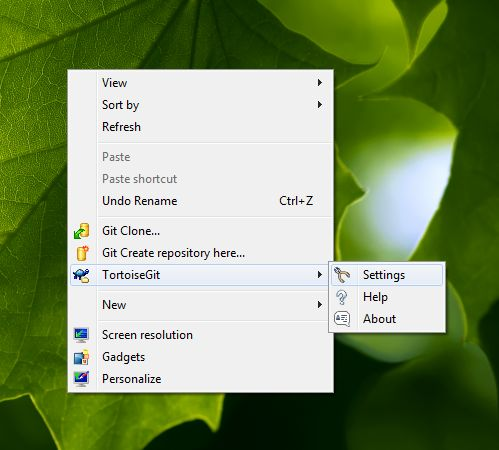
\includegraphics[scale=0.5]{../IMG/settingsTG.jpg}
	\end{center}
	\caption{Le menu de Tortoise Git}
	\label{Le menu de Tortoise Git} 
\end{figure}

Allez dans Tortoise Git $\rightarrow$ Settings $\rightarrow$ Git\\

Ici, vous verrez un menu "User info", vous allez remplir le champ "Name" et "Email".
Le bouton Edit global .gitconfig vous permet de voir le résultat (cf. "Par fichier")

\newpage
\section{Création d'un dépôt avec github}

Connectez-vous sur le site et allez dans "New repository".
Renseignez le nom du projet puis Create repository (sans .gitignore ni license).\\

\begin{figure}[h] 
	\begin{center}
		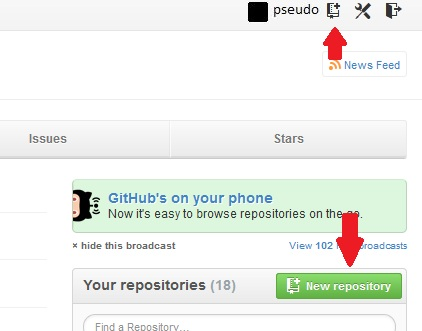
\includegraphics[scale=0.6]{../IMG/githubcreate.jpg}
	\end{center}
	\caption{GitHub : creer un depot}
	\label{GitHub : creer un depot} 
\end{figure}

\textbf{Attention :} Par défaut les dépôts sont publics.\\
Sous github : ne mettez \textbf{aucune} information confidentielle.